\documentclass[10pt]{article}
\usepackage[margin=0.75in]{geometry}
\usepackage{amsmath,amssymb}
\usepackage{xcolor}
\usepackage{tikz}
\usetikzlibrary{arrows.meta,fit,backgrounds}
\definecolor{sentcolor}{HTML}{A65313}
\definecolor{computedcolor}{HTML}{235D8C}
\tikzset{value/.style={draw,rounded corners=2pt,minimum width=7mm,minimum height=4.5mm,inner sep=2pt,font=\scriptsize},sent/.style={value,draw=sentcolor,fill=sentcolor!10,double,double distance=.6pt},computed/.style={value,draw=computedcolor,fill=computedcolor!8},unused/.style={value,draw=black!25,text=black!45,fill=black!3},active edge/.style={-{Latex[length=1.5mm]},draw=computedcolor,semithick},unused edge/.style={-{Latex[length=1.5mm]},draw=black!25,dashed},group/.style={draw=black!25,rounded corners=3pt,dashed,inner sep=5pt},diagram label/.style={font=\scriptsize,align=center}}
\newcommand{\seeddiagram}[1]{%
\begin{tikzpicture}[x=.95cm,y=.8cm]
 \ifnum#1=2 \def\blocks{1/0,2/3.6}\def\rooty{.2}\def\bottomy{-3.1}\def\rootinputs{12}\def\rootunits{3}\def\remaining{11}\else \def\blocks{1/0}\def\rooty{1}\def\bottomy{-1.6}\def\rootinputs{18}\def\rootunits{5}\def\remaining{17}\fi
 \foreach \i in {1,...,4} {
   \def\gap{0}\ifnum#1=2 \ifnum\i>2 \def\gap{1.6}\fi\fi
   \pgfmathsetmacro{\rowy}{3.5-\i-\gap}
   \def\ts{computed}\ifnum\i=4 \def\ts{sent}\fi
   \node[\ts] (t-\i) at (6.2,\rowy) {$t_\i$};
   \foreach \j in {1,...,4} {
     \ifnum#1=2
       \ifnum\i<3 \ifnum\j=3 \def\ls{sent}\else \def\ls{computed}\fi\else \ifodd\j \def\ls{sent}\else \def\ls{computed}\fi\fi
     \else
       \ifnum\j<3 \def\ls{computed}\else \def\ls{sent}\fi
     \fi
     \ifnum\i=4 \def\ls{unused}\fi
     \node[\ls] (l-\i-\j) at ({1.4*(\j-1)},\rowy) {$\ell_{\i\j}$};
   }
 }
 \foreach \b/\offset in \blocks {
   \pgfmathtruncatemacro{\firstrow}{#1*(\b-1)+1}
   \pgfmathtruncatemacro{\lastrow}{#1*\b}
   \pgfmathsetmacro{\lasty}{3.5-\lastrow-(#1==2 && \b==2 ? 1.6 : 0)}
   \foreach \j in {1,...,4} {
     \def\revealseed{0}
     \ifnum#1=2
       \ifnum\b=1 \ifnum\j=3\else \def\revealseed{1}\fi\else \ifodd\j\else \def\revealseed{1}\fi\fi
     \else
       \ifnum\j<3 \def\revealseed{1}\fi
     \fi
     \ifnum\revealseed=1 \def\ss{sent}\def\edgekind{active edge}\def\buscolor{computedcolor}\else \def\ss{unused}\def\edgekind{unused edge}\def\buscolor{black!25}\fi
     \ifnum#1=2 \def\seedlabel{s_{\b\j}}\else \def\seedlabel{s_\j}\fi
     \node[\ss] (s-\b-\j) at ({1.4*(\j-1)},{4.1-\offset}) {$\seedlabel$};
     \node[text=\buscolor,inner sep=1pt,font=\scriptsize] (h-\b-\j) at ({1.4*(\j-1)},{3.4-\offset}) {$H_{#1}$};
     \draw[\edgekind] (s-\b-\j)--(h-\b-\j);
     \draw[draw=\buscolor] (h-\b-\j.east)--({1.4*(\j-1)+.62},{3.4-\offset})--({1.4*(\j-1)+.62},\lasty);
     \foreach \i in {\firstrow,...,\lastrow} {
       \def\gap{0}\ifnum#1=2 \ifnum\i>2 \def\gap{1.6}\fi\fi
       \pgfmathsetmacro{\rowy}{3.5-\i-\gap}
       \fill[\buscolor] ({1.4*(\j-1)+.62},\rowy) circle[radius=.7pt];
       \draw[\edgekind] ({1.4*(\j-1)+.62},\rowy)--(l-\i-\j.east);
     }
   }
 }
 \foreach \i in {1,...,4} {
   \def\gap{0}\ifnum#1=2 \ifnum\i>2 \def\gap{1.6}\fi\fi
   \pgfmathsetmacro{\rowy}{3.5-\i-\gap}
   \def\edgekind{active edge}\ifnum\i=4 \def\edgekind{unused edge}\fi
   \foreach \j in {1,...,4} {
     \draw[\edgekind,rounded corners=2pt] (l-\i-\j.south)--({1.4*(\j-1)},{\rowy-.27-.10*\j})--(5.5,{\rowy-.27-.10*\j})--(t-\i.west);
   }
 }
 \node[diagram label] at (6.2,4.1) {Row hashes\\$4n\to n$};
 \node[computed] (g) at (8.3,\rooty) {$g$};
 \node[diagram label,above=4pt] at (g.north) {$4n\to n$\\1 unit};
 \node[computed,minimum width=12mm] (pk) at (10.8,\rooty) {$\mathsf{pk}$};
 \node[diagram label,right=4pt] at (pk.east) {$\rootinputs n\to n$\\\rootunits\ units};
 \foreach \i in {1,...,4} {\draw[active edge] (t-\i.east)--(g.west);}
 \draw[active edge] (g)--(pk);
 \node[diagram label] (more) at (8.6,\bottomy) {\remaining\ further\\component roots};
 \draw[active edge,dotted] (more.east) to[out=0,in=-90] (pk.south);
\end{tikzpicture}%
}
\usepackage[hidelinks]{hyperref}
\newcommand{\roinput}{N_{\mathrm{RO,input}}}
\newcommand{\rooutput}{N_{\mathrm{RO,output}}}
\newcommand{\keybudget}{N_{\mathrm{RO,keygen}}^{\max}}
\newcommand{\gamebudget}{N_{\mathrm{RO,game}}^{\max}}
\newcommand{\fieldbudget}{N_{\mathrm{frontier}}^{\max}}
\newcommand{\sigbudget}{S_{\mathrm{sig}}^{\max}}
\newcommand{\cutbudget}{N_{\mathrm{cuts}}}
\newcommand{\grinding}{n_{\mathrm{grinding}}}
\newcommand{\hashcost}{c_{\mathrm{hash}}}
\newcommand{\reconstructcost}{C_{\mathrm{reconstruct}}}
\title{looking for the optimal hash-based one-time signature}
\author{}
\date{}
\begin{document}
\maketitle
\vspace{-2em}

We restrict attention to one-time signatures that reveal values from a precomputed hash graph to reconstruct a public root. Within this class, we seek the least verification cost under key-generation and signature-size budgets.

\section{The framework}
\paragraph{Hashes and keys.} Fix a digest size $n\ge2$, integer capacities $\roinput,\rooutput\ge1$ in $n$-bit blocks, and a public space $\mathcal T$ of hash addresses (tweaks). Our oracle is
\[
 H_\ell:\mathcal T\times\bigcup_{k\ge1}\{0,1\}^{kn}\longrightarrow\{0,1\}^{\ell n},\qquad 1\le\ell\le\rooutput,\qquad \hashcost(k)=\left\lceil k/\roinput\right\rceil.
\]
Each tweak--input pair determines an independent uniform $\rooutput n$-bit string; $H_\ell$ returns its first $\ell$ blocks. A $kn$-bit input costs $\hashcost(k)$ units, independently of $\ell$. Write $H=H_1$. Sampling, storage, and other computation are free.

Fix an acyclic hash graph~\cite{BM94}. A \emph{vertex} carries one $n$-bit value; a \emph{gate} is one hash call with ordered inputs and outputs. Gates have distinct tweaks, and each nonsource vertex has one producer. Sample independent $n$-bit sources, compute and store all values, and publish the root. Sizes are in bits; $N,S$ denote fixed parameters or budgets, $C$ costs determined by the graph and disclosure, and $X$ random call counts.

\paragraph{Disclosures.} A disclosure $D$ is an ordered list of vertices whose values reconstruct the root by graph evaluation; $|D|$ is the number of transmitted $n$-bit values. It must be \emph{minimal}: removing any listed vertex prevents reconstruction. Fix a public schedule using every disclosed value and evaluating each needed gate once. These are structural requirements; the public root is used only for the final comparison.

\paragraph{Costs.} Let $\mathcal G$ be the set of all graph gates, $k_g$ the number of $n$-bit input blocks to gate $g$, and $\mathcal G(D)$ the gates in the reconstruction schedule for $D$. Define
\[
 C_{\mathrm{keygen}}=\sum_{g\in\mathcal G}\hashcost(k_g),\qquad \reconstructcost(D)=\sum_{g\in\mathcal G(D)}\hashcost(k_g).
\]
Thus $\reconstructcost(D)$ is the cost of reconstructing the root from $D$, including seed expansions and the final root hash, but excluding message encoding. A gate is charged once even if its outputs are reused. Require $C_{\mathrm{keygen}}\le\keybudget$, where $\keybudget$ is the fixed key-generation cost budget.

\paragraph{Codebook.} Let $\sigbudget$ be the signature-size budget in bits and set $\fieldbudget=\lfloor\sigbudget/n\rfloor-2$ to reserve space for the $2n$-bit nonce. Fix a public ordered codebook of $\cutbudget=2^{n-1-\grinding}$ disclosures independently of the oracle, with integer $0\le\grinding\le n-1$. Require $|D|\le\fieldbudget$ and a common positive reconstruction cost for every disclosure. Require \emph{incomparability}: no disclosure can produce another by forward hashing. Tree cuts meet every root-to-leaf path once; they are minimal and incomparable at equal reconstruction cost. We check shared seeds below.

\paragraph{Sign once.} Given a $2n$-bit message $m$, try distinct uniform $2n$-bit nonces $\eta$. Interpret all $n$ bits of $H(\tau_{\mathrm{enc}},m\Vert\eta)$ as an integer $d$, using a reserved tweak. If $d<\cutbudget$, send $\eta$ and the stored values of disclosure $d$. Otherwise retry, returning $\bot$ after a fixed limit $1\le N_{\mathrm{trials}}^{\max}\le2^{2n}$. Let $X_{\mathrm{RO,sign}}$ count these encoding queries. For a message fixed independently of the encoding oracle,
\[
 p=\cutbudget/2^n=2^{-\grinding-1},\qquad \mathbb E[X_{\mathrm{RO,sign}}]\le1/p,\qquad \Pr[\bot]=(1-p)^{N_{\mathrm{trials}}^{\max}}.
\]
\paragraph{Verify.} Recompute $d$; reject invalid indices or any incorrect field count or length. Run the schedule for the selected disclosure $D$ and accept exactly when the reconstructed root matches the public key. The signature contains the nonce and $|D|$ values; verification adds one $4n$-bit message-and-nonce encoding query to reconstruction:
\[
 |\sigma|=(2+|D|)n\le\sigbudget,\qquad C_{\mathrm{verif}}(D)=\reconstructcost(D)+\hashcost(4).
\]
The codebook makes $C_{\mathrm{verif}}(D)$ constant on valid signatures; write $C_{\mathrm{verif}}$ for this common cost.
\paragraph{Security target.} In a freshly sampled random oracle, a classical adversary receives the public key, accesses the oracle, makes at most one adaptive signing request, and wins by producing an accepted $(m,\sigma)$ pair never returned by the signer: \emph{strong one-time unforgeability}. For every such adversary and integer $\gamebudget\ge1$ bounding the entire experiment's cost on every execution path, the $n-1$-bit target is $\Pr[\mathrm{Forge}]\le\gamebudget/2^{n-1}$. Charge all queries by $\hashcost(k)$, including preprocessing, key generation, signing, adversarial queries, and final verification. Probability covers all randomness. This bound remains unproved; the results below establish combinatorial counts and costs.

\paragraph{Counting and decoding.} In a counting polynomial $P(x,y)$, $[x^cy^f]P$ counts disclosures with reconstruction cost $c$ and $f$ transmitted values. Represent each choice by $x^cy^f$, add alternatives, and multiply independent choices. Local polynomials count only reconstruction within the indicated part of the graph; subsequent hashes are charged separately. Keep the first $\cutbudget$ eligible disclosures in a fixed order. Decode an index by counting valid completions of each local choice, selecting its index block, subtracting earlier block sizes, and repeating. No vertex identifiers or extra oracle queries are needed.

The illustration shows one possible disclosure in an irregular graph. Key generation samples the source secrets $s_i$ and evaluates the whole graph. For this signature, the verifier receives the orange values, computes the blue parts, and checks the reconstructed root against the public key; the gray parts are unused.

\begin{center}
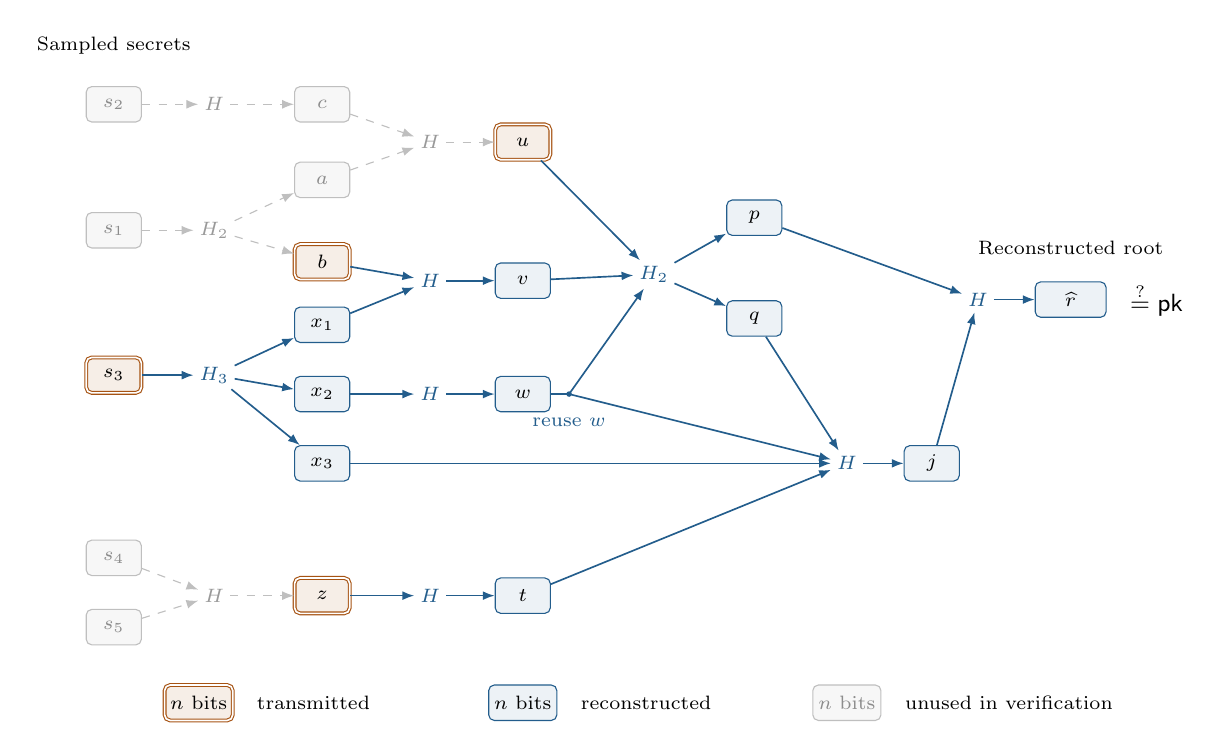
\begin{tikzpicture}[x=.98cm,y=.8cm]
 \node[unused] (s2) at (0,6.8) {$s_2$};
 \node[unused] (s1) at (0,4.8) {$s_1$};
 \node[sent] (s3) at (0,2.5) {$s_3$};
 \node[unused] (s4) at (0,-.4) {$s_4$};
 \node[unused] (s5) at (0,-1.5) {$s_5$};
 \node[diagram label,above=8pt] at (s2.north) {Sampled secrets};

 \node[unused] (c) at (2.7,6.8) {$c$};
 \node[unused] (a) at (2.7,5.6) {$a$};
 \node[sent] (b) at (2.7,4.3) {$b$};
 \node[computed] (d) at (2.7,3.3) {$x_1$};
 \node[computed] (e) at (2.7,2.2) {$x_2$};
 \node[computed] (f) at (2.7,1.1) {$x_3$};
 \node[sent] (z) at (2.7,-1) {$z$};

 \node[sent] (u) at (5.3,6.2) {$u$};
 \node[computed] (v) at (5.3,4) {$v$};
 \node[computed] (w) at (5.3,2.2) {$w$};
 \node[computed] (t) at (5.3,-1) {$t$};
 \node[computed] (p) at (8.3,5) {$p$};
 \node[computed] (q) at (8.3,3.4) {$q$};
 \node[computed] (j) at (10.6,1.1) {$j$};
 \node[computed,minimum width=9mm] (r) at (12.4,3.7) {$\widehat r$};
 \node[diagram label,above=6pt] at (r.north) {Reconstructed root};
 \node[font=\small,right=5pt] at (r.east) {$\stackrel{?}{=}\mathsf{pk}$};

 % Hash operations are bare labels; only digest values have boxes.
 \node[text=black!40,font=\scriptsize,inner sep=2pt] (hc) at (1.3,6.8) {$H$};
 \node[text=black!40,font=\scriptsize,inner sep=2pt] (hab) at (1.3,4.8) {$H_2$};
 \node[text=black!40,font=\scriptsize,inner sep=2pt] (hu) at (4.1,6.2) {$H$};
 \node[text=black!40,font=\scriptsize,inner sep=2pt] (hz) at (1.3,-1) {$H$};
 \node[text=computedcolor,font=\scriptsize,inner sep=2pt] (hdef) at (1.3,2.5) {$H_3$};
 \node[text=computedcolor,font=\scriptsize,inner sep=2pt] (hv) at (4.1,4) {$H$};
 \node[text=computedcolor,font=\scriptsize,inner sep=2pt] (hw) at (4.1,2.2) {$H$};
 \node[text=computedcolor,font=\scriptsize,inner sep=2pt] (ht) at (4.1,-1) {$H$};
 \node[text=computedcolor,font=\scriptsize,inner sep=2pt] (hpq) at (7,4.1) {$H_2$};
 \node[text=computedcolor,font=\scriptsize,inner sep=2pt] (hj) at (9.5,1.1) {$H$};
 \node[text=computedcolor,font=\scriptsize,inner sep=2pt] (hr) at (11.2,3.7) {$H$};

 \foreach \src/\dst in {s2/hc,hc/c,s1/hab,hab/a,hab/b,a/hu,c/hu,hu/u,s4/hz,s5/hz,hz/z} {\draw[unused edge] (\src)--(\dst);}
 \foreach \src/\dst in {s3/hdef,hdef/d,hdef/e,hdef/f,b/hv,d/hv,hv/v,e/hw,hw/w,z/ht,ht/t,u/hpq,v/hpq,hpq/p,hpq/q,q/hj,f/hj,t/hj,hj/j,p/hr,j/hr,hr/r} {\draw[active edge] (\src)--(\dst);}
 \coordinate (reuse) at (5.9,2.2);
 \draw[draw=computedcolor,semithick] (w.east)--(reuse);
 \fill[computedcolor] (reuse) circle[radius=1pt];
 \draw[active edge] (reuse)--(hpq);
 \draw[active edge] (reuse)--(hj);
 \node[diagram label,text=computedcolor,below=5pt] at (reuse) {reuse $w$};

 \node[sent] (legend-sent) at (1.1,-2.7) {$n$ bits};
 \node[diagram label,right=5pt] at (legend-sent.east) {transmitted};
 \node[computed] (legend-computed) at (5.3,-2.7) {$n$ bits};
 \node[diagram label,right=5pt] at (legend-computed.east) {reconstructed};
 \node[unused] (legend-unused) at (9.5,-2.7) {$n$ bits};
 \node[diagram label,right=5pt] at (legend-unused.east) {unused in verification};
\end{tikzpicture}
\end{center}

Each box holds one $n$-bit value. A bare $H_\ell$ label is one hash call producing $\ell$ values; $H=H_1$. At each hash label, inputs and outputs are ordered from top to bottom; distinct tweaks are omitted. The two arrows leaving $w$ reuse the same value. This illustration uses up to three output blocks per call.

Hash a $2n$-bit message $m$ with a $2n$-bit nonce $\eta$ to select a disclosure from a fixed codebook; retry when the hash is not accepted. For the highlighted disclosure,
\[
 (m,\eta)\xrightarrow{H(\tau_{\mathrm{enc}},m\Vert\eta)}d\xrightarrow{\text{codebook}}D_d=(u,b,s_3,z),\qquad \sigma=(\eta,\textcolor{sentcolor}{u,b,s_3,z}).
\]
Every highlighted value is needed; neither the graph nor vertex identifiers are sent. With $\roinput=4$, all drawn calls cost one unit: the whole graph has $C_{\mathrm{keygen}}=11$, the seven blue calls give $\reconstructcost(D_d)=7$, and encoding gives $C_{\mathrm{verif}}(D_d)=8$. The signature has $(2+4)n=6n$ bits.

\clearpage
\section{Four constructions under the same budgets}
Take
\[
 n=128,\quad \grinding=15,\quad \roinput=\rooutput=4,\quad \keybudget=168,\quad \fieldbudget=128.
\]
We need $2^{112}$ disclosures. Every scheme has a 128-bit public key, signatures of at most $130n=16640$ bits, and at most $2^{16}$ expected signing queries. Encoding costs one verification unit. The constructions below use \textbf{73, 68, 63, and 60 verification units}.

In the drawings, orange double boxes are transmitted values, blue parts are computed, and gray parts are unused during verification. A merge hashes all incoming values together; an $H_\ell$ gate produces $\ell$ values in one query. Crossings connect only where marked with a dot. Repeated parts are labeled with their actual counts.

\subsection{Top-of-the-hypercube chains: 73 units}
A chain repeatedly hashes a secret to an endpoint. Revealing an intermediate value lets the verifier advance to that endpoint. Join several chains by hashing their endpoints into the public key. The signature sends one value per chain; choose positions with a fixed sum of remaining distances. This is the top-layer encoding of Khovratovich et al.~\cite{hypercube}.

Use 23 chains of length two and 93 of length one, with total remaining distance 43. In the drawing, $s_i$ is a secret, $u_i$ an intermediate value, and $e_i$ an endpoint. The six illustrated distances are $2,1,0,1,0,1$.

\begin{center}
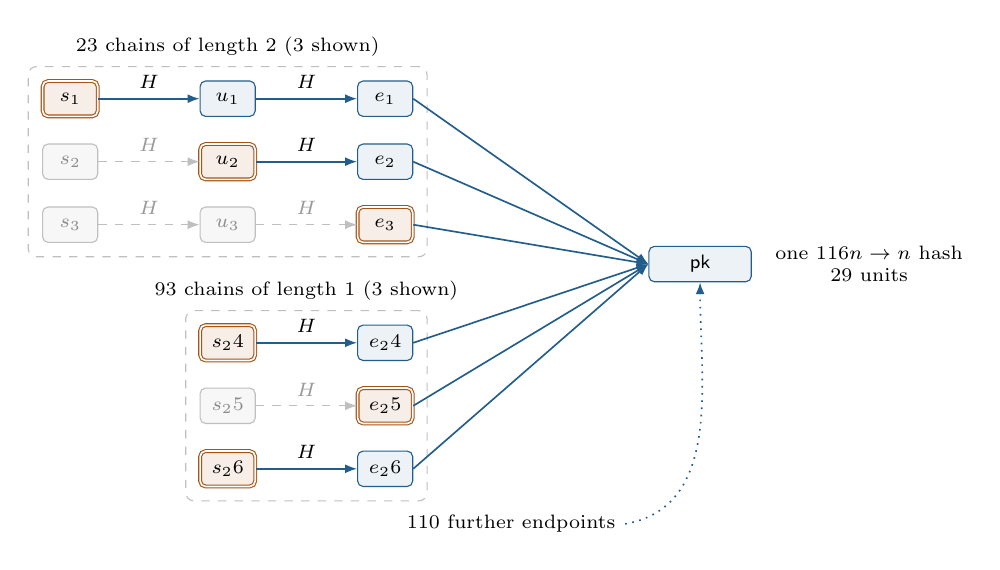
\begin{tikzpicture}[x=1cm,y=1cm]
 \node[computed,minimum width=13mm] (pk) at (8,2.2) {$\mathsf{pk}$};
 \node[diagram label,right=5pt] at (pk.east) {one $116n\to n$ hash\\29 units};
 \foreach \i/\yy in {1/4.3,2/3.5,3/2.7} {
   \ifnum\i=1 \def\ss{sent}\def\us{computed}\def\es{computed}\else\ifnum\i=2 \def\ss{unused}\def\us{sent}\def\es{computed}\else \def\ss{unused}\def\us{unused}\def\es{sent}\fi\fi
   \node[\ss] (s\i) at (0,\yy) {$s_\i$};
   \node[\us] (u\i) at (2,\yy) {$u_\i$};
   \node[\es] (e\i) at (4,\yy) {$e_\i$};
   \ifnum\i=1 \draw[active edge] (s\i)--node[above,font=\scriptsize] {$H$} (u\i);\else \draw[unused edge] (s\i)--node[above,font=\scriptsize,text=black!40] {$H$} (u\i);\fi
   \ifnum\i=3 \draw[unused edge] (u\i)--node[above,font=\scriptsize,text=black!40] {$H$} (e\i);\else \draw[active edge] (u\i)--node[above,font=\scriptsize] {$H$} (e\i);\fi
   \draw[active edge] (e\i.east)--(pk.west);
 }
 \foreach \i/\yy in {24/1.2,25/.4,26/-.4} {
   \ifnum\i=25 \def\ss{unused}\def\es{sent}\else \def\ss{sent}\def\es{computed}\fi
   \node[\ss] (s\i) at (2,\yy) {$s_\i$};
   \node[\es] (e\i) at (4,\yy) {$e_\i$};
   \ifnum\i=25 \draw[unused edge] (s\i)--node[above,font=\scriptsize,text=black!40] {$H$} (e\i);\else \draw[active edge] (s\i)--node[above,font=\scriptsize] {$H$} (e\i);\fi
   \draw[active edge] (e\i.east)--(pk.west);
 }
 \node[diagram label] (more) at (5.6,-1.1) {110 further endpoints};
 \draw[active edge,dotted] (more.east) to[out=10,in=-90] (pk.south);
 \begin{scope}[on background layer]
   \node[group,fit=(s1)(e3),label={[diagram label]above:23 chains of length 2 (3 shown)}] {};
   \node[group,fit=(s24)(e26),label={[diagram label]above:93 chains of length 1 (3 shown)}] {};
 \end{scope}
\end{tikzpicture}
\end{center}

Let $G_L(x)=1+x+\cdots+x^L$ count positions in a length-$L$ chain. There are enough disclosures because $[x^{43}]G_2^{23}G_1^{93}>2^{112}$. Building the chains costs $23\cdot2+93=139$ units; the $116n\to n$ root hash costs 29. Hence
\[
 C_{\mathrm{keygen}}=139+29=168,\qquad |\sigma|=118n,\qquad C_{\mathrm{verif}}=43+29+1=\mathbf{73}.
\]
\paragraph{Why this is optimal among chains.} For fixed total length and number of chains, balanced lengths maximize every coefficient: for $b\ge a+2$,
\[
 G_{a+1}G_{b-1}-G_aG_b=x^{a+1}G_{b-a-2}\ge0.
\]
Extra length cannot hurt. With $t$ chains, spend the available $168-\lceil t/4\rceil$ unary hashes on balanced lengths: put $\lambda_t=\lfloor(168-\lceil t/4\rceil)/t\rfloor$ and $a_t=168-\lceil t/4\rceil-t\lambda_t$. Exact coefficient expansion gives
\[
 \max_{1\le t\le128}[x^{71-\lceil t/4\rceil}]G_{\lambda_t}^{t-a_t}G_{\lambda_t+1}^{a_t}<2^{112}.
\]
These coefficient sequences are symmetric and unimodal; their midpoints correspond to reconstruction costs above 71. Thus no disclosure layer with reconstruction cost at most 71 supplies enough choices: the minimum verification cost, including encoding, is 73 units.

\clearpage
\subsection{A branching forest: 68 units}
Group four one-step chains into a component: hash secrets $s_{ji}$ into endpoints $e_{ji}$, then hash the four endpoints into a component root $g_j$. Use 32 independent components and hash their roots into the public key.

A disclosure may send a component root directly, or expand it and send one value from each of its four chains. Branching therefore adds a choice of which components to expand. The drawing shows three possibilities on the same underlying shape.

\begin{center}
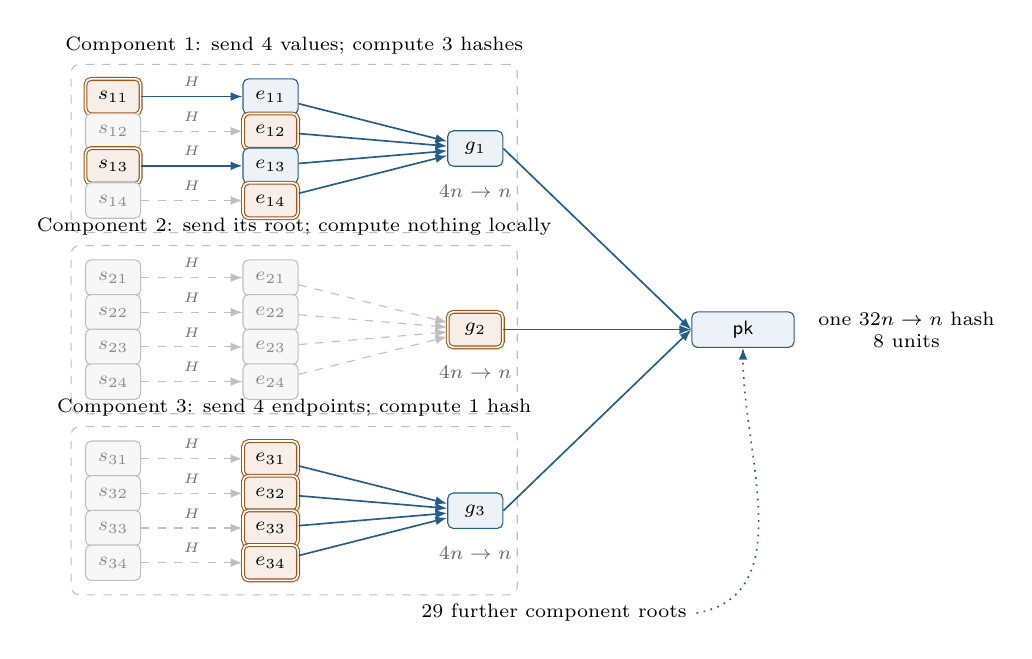
\begin{tikzpicture}[x=1cm,y=1cm]
 \node[computed,minimum width=13mm] (pk) at (8,2.3) {$\mathsf{pk}$};
 \node[diagram label,right=5pt] at (pk.east) {one $32n\to n$ hash\\8 units};
 \foreach \j/\yy in {1/4.6,2/2.3,3/0} {
   \ifnum\j=2 \def\gs{sent}\else \def\gs{computed}\fi
   \node[\gs] (g\j) at (4.6,\yy) {$g_\j$};
   \node[diagram label,below=3pt,text=black!60] at (g\j.south) {$4n\to n$};
   \foreach \i/\dy in {1/.66,2/.22,3/-.22,4/-.66} {
     \def\ss{unused}\def\es{sent}
     \ifnum\j=2 \def\es{unused}\fi
     \ifnum\j=1 \ifodd\i \def\ss{sent}\def\es{computed}\fi\fi
     \node[\ss] (s\j\i) at (0,{\yy+\dy}) {$s_{\j\i}$};
     \node[\es] (e\j\i) at (2,{\yy+\dy}) {$e_{\j\i}$};
     \def\edgekind{unused edge}
     \ifnum\j=1 \ifodd\i \def\edgekind{active edge}\fi\fi
     \draw[\edgekind] (s\j\i)--node[above,font=\tiny,text=black!55] {$H$} (e\j\i);
     \ifnum\j=2 \draw[unused edge] (e\j\i)--(g\j);\else \draw[active edge] (e\j\i)--(g\j);\fi
   }
   \draw[active edge] (g\j.east)--(pk.west);
 }
 \node[diagram label] (more) at (5.6,-1.3) {29 further component roots};
 \draw[active edge,dotted] (more.east) to[out=10,in=-90] (pk.south);
 \begin{scope}[on background layer]
   \node[group,fit=(s11)(s14)(g1),label={[diagram label]above:Component 1: send 4 values; compute 3 hashes}] {};
   \node[group,fit=(s21)(s24)(g2),label={[diagram label]above:Component 2: send its root; compute nothing locally}] {};
   \node[group,fit=(s31)(s34)(g3),label={[diagram label]above:Component 3: send 4 endpoints; compute 1 hash}] {};
 \end{scope}
\end{tikzpicture}
\end{center}

The local counting polynomial is
\[
 P_{\mathrm{forest}}(x,y)=\underbrace{y}_{\text{send the root}}+\underbrace{xy^4(1+x)^4}_{\text{expand the root, then choose four chain positions}}.
\]
Each component costs five units to build and sends at most four values. Choose disclosures for which reconstructing the 32 component roots costs 59 in total. Since $[x^{59}]P_{\mathrm{forest}}(x,1)^{32}>2^{112}$, this supplies the codebook, with at most 128 values. The final $32n\to n$ hash costs eight units, giving
\[
 C_{\mathrm{keygen}}=32\cdot5+8=168,\qquad C_{\mathrm{verif}}=59+8+1=\mathbf{68}.
\]
This improves on the optimal chain baseline; optimality among all trees is not claimed.

\clearpage
\subsection{Pairwise shared seeds: 63 units}
Derive two leaves from one secret seed and reveal the seed when both leaves are needed.\footnote{This idea was suggested by Justin Drake.} This replaces two transmitted values with one, at the cost of one expansion query. Here the paired leaves belong to different authentication rows, so one seed helps reconstruct two row hashes.

Arrange sixteen leaves in four rows of four. Hash each row into $t_i$, then hash the four row roots into a component root $g$. Four seeds supply rows 1 and 2; four independent seeds supply rows 3 and 4:
\[
 H_2(\tau^s_{bj},s_{bj})=\ell_{2b-1,j}\Vert\ell_{2b,j}\quad(b=1,2;\ j=1,\ldots,4),\qquad t_i=H(\tau^t_i,\ell_{i1}\Vert\cdots\Vert\ell_{i4}),\qquad g=H(\tau_g,t_1\Vert\cdots\Vert t_4).
\]
For rows 1--2, reveal seeds in columns 1, 2, and 4; for row 3, reveal seeds in columns 2 and 4. Send the missing leaves and $t_4$. This supplies five seeds, four leaves, and one row root. Reconstructing $g$ takes five seed expansions, three row hashes, and one final hash: nine units.
\begin{center}
\seeddiagram{2}
\end{center}

\paragraph{One counting rule for shared seeds.} Consider a group of $r$ rows sharing four seeds, one per column; here $r=2$, and the next construction uses $r=4$. Choose $1\le k\le r$ rows to recompute and $0\le q\le3$ seeds to reveal. Send the other $r-k$ row roots, the $q$ seeds, and the $k(4-q)$ leaves still missing from the chosen rows. The verifier uses $q$ seed expansions and $k$ row hashes. Also allow sending all row roots, or all four seeds. These choices give
\[
 Q_r(x,y)=y^r+x^{r+4}y^4+\sum_{k=1}^r\sum_{q=0}^3\binom rk\binom4q x^{k+q}y^{(r-k)+q+k(4-q)}.
\]
Every listed disclosure is minimal: removing a row root leaves an unreconstructible row, and removing a leaf or seed leaves a required column input missing. Forward hashing can only remove disclosed seeds and, while any seed is missing, can only remove expanded rows. Every strict change lowers reconstruction cost; the all-seed disclosure has the unique maximum cost $r+4$. Consequently, disclosures of equal reconstruction cost are incomparable, including across independent groups and components.

For pairs, the full component polynomial is $P_{\mathrm{pairs}}=y+xQ_2^2$: send $g$, or compute it from two independent row pairs. Use 12 components, each costing eight seed expansions and five combining hashes to build. The exact count
\[
 \sum_{f=1}^{128}[x^{59}y^f]P_{\mathrm{pairs}}(x,y)^{12}>2^{112}
\]
provides the codebook. The final $12n\to n$ hash costs three units, so
\[
 C_{\mathrm{keygen}}=12\cdot13+3=159\le168,\qquad C_{\mathrm{verif}}=59+3+1=\mathbf{63}.
\]

\clearpage
\subsection{Seeds shared by four leaves: 60 units}
Keep the same four rows, but let each seed generate a whole column:
\[
 H_4(\tau^s_j,s_j)=\ell_{1j}\Vert\ell_{2j}\Vert\ell_{3j}\Vert\ell_{4j}\quad(j=1,\ldots,4).
\]
The row hashes $t_i$ and component root $g$ are unchanged. Each component now needs four seed expansions and five combining hashes to build, costing nine units. A revealed seed can replace one leaf in each row being reconstructed: with $k$ such rows, it saves $(k-1)n$ signature bits for one extra query.

For example, send $t_4$ and reconstruct rows 1--3. Seeds $s_1,s_2$ supply the first two columns, leaving six individual leaves to send. The disclosure therefore contains $1+2+6=9$ values. Computing $g$ takes two expansions, three row hashes, and one final hash: six units.
\begin{center}
\seeddiagram{4}
\end{center}

The same counting rule now uses $r=4$. The component polynomial is $P_{\mathrm{four}}=y+xQ_4$: send $g$, or reconstruct it from the four rows. Use 18 components and select disclosures for which reconstructing the component roots costs 54 in total, with at most 128 values. There are enough because
\[
 \sum_{f=1}^{128}[x^{54}y^f]P_{\mathrm{four}}(x,y)^{18}>2^{112}.
\]
The final $18n\to n$ hash costs five units. Thus the same public-key and signature-size bounds are met with
\[
 C_{\mathrm{keygen}}=18\cdot9+5=167\le168,\qquad C_{\mathrm{verif}}=54+5+1=\mathbf{60}.
\]
\begin{thebibliography}{KKW25}
\bibitem[BM94]{BM94} Daniel Bleichenbacher and Ueli~M. Maurer. Directed acyclic graphs, one-way functions and digital signatures. In Yvo Desmedt, editor, \emph{Advances in Cryptology---CRYPTO '94}, volume 839 of \emph{LNCS}, pages 75--82. Springer, 1994. \url{https://crypto.ethz.ch/publications/files/BleMau94.pdf}.
\bibitem[KKW25]{hypercube} Dmitry Khovratovich, Mikhail Kudinov, and Benedikt Wagner. At the top of the hypercube---better size-time tradeoffs for hash-based signatures. In \emph{Advances in Cryptology---CRYPTO 2025, Part VI}, volume 16005 of \emph{LNCS}, pages 93--123. Springer, 2025. Full version: IACR Cryptology ePrint Archive, Report 2025/889. \url{https://eprint.iacr.org/2025/889}.
\end{thebibliography}
\end{document}
